\chapter{Descripción del proyecto}
\label{chap:Problema}
\textit{The first chapter introduces fluorescence-based DNA technology and highlights the motivation of the research conducted in the thesis}
\vfill
\minitoc
\newpage

\section{Definición del problema}
  \paragraph*{}
  Una de las mayores ventajas competitivas en una empresa es que la gestión de todos sus procesos y componentes estén alineados con su estrategia empresarial y su filosofía corporativa, sin embargo, realizar este proceso requiere una metodología que asegure que su planteamiento es efectivo. \\
  Creatics es una empresa en proceso de creación que requiere establecer estrategias de competitividad y sostenibilidad que la hagan desde el inicio una empresa sólida.

\section{Formulación del problema}
  \paragraph*{}
  ¿Es la Arquitectura Empresarial la metodología que permita alinear los procesos y componentes del producto mistituto.com de la empresa Creatics con el cumplimiento de sus objetivos estratégicos?

\section{Objetivos}
  \subsection{Objetivo General}
    \paragraph*{}
    Desarrollar una Arquitectura Empresarial para el producto mistituto.com de la empresa Creatics utilizando como herramienta el lenguaje de Arquitectura Archimate.

  \subsection{Objetivos Específicos}
    \begin{itemize}
      \item Identificar la filosofía y características organizacionales de Creatics.
      \item Establecer actores, roles y stakeholders dentro de los diferentes procesos.
      \item Determinar los procesos, datos, aplicaciones, infraestructura tecnológica y demás componentes para la modelación.
    \end{itemize}

\section{Alcance}
  \paragraph*{}
  Se desarrollará la Arquitectura Empresarial para el producto minstituto.com de la empresa Creatics utilizando el lenguaje de arquitectura Archimate.

\chapter{Presentación de la organización}
\label{chap:Descripcion}
\textit{The first chapter introduces fluorescence-based DNA technology and highlights the motivation of the research conducted in the thesis}
\vfill
\minitoc
\newpage

\section{Filosofía Organizacional}
  
  \subsection{Misión}
    \paragraph*{}
    Generamos soluciones tecnológicas que promueven el progreso de nuestros clientes contando con un equipo de trabajo altamente competitivo.
  
  \subsection{Visión}
    \paragraph*{}
    Ser reconocidos por nuestros productos innovadores principalmente en el sector de instituciones educativas.
  
  \subsection{Objetivos estratégicos}
    \begin{itemize}
  	  \item Proveer soluciones tecnológicas que permitan optimizar la gestión de la información en las instituciones educativas, generando renta para nuestros socios.
      \item Generar reconocimiento en el sector de instituciones educativas.
    \end{itemize}

  \subsection{Principios}
    \begin{itemize}
    	\item \textbf{Compromiso:} Orientamos nuestros esfuerzos al cumplimiento de las metas establecidas.
    	\item \textbf{Innovación:} Buscamos generar valor agregado a nuestros productos que permitan incrementar los beneficios a nuestros clientes.
    	\item \textbf{Enfoque al cliente:} Nuestros procesos se orientan en ofrecer el mejor servicio siendo respaldo para nuestros clientes.
    	\item \textbf{Confidencialidad:} Nuestros clientes cuentan con la garantía de que su información no será divulgada y tendrán un manejo apropiado de la información de su organización.
    	\item \textbf{Responsabilidad social y ambiental:} Buscamos beneficiar a nuestros colaboradores y a la sociedad al igual que el medio ambiente por medio de nuestros procesos internos.
    \end{itemize}
    
    \subsection{Valores}
      \begin{itemize}
		\item \textbf{Respeto:} Consiste en reconocer, aceptar y comprender los intereses y necesidades de todos los integrantes de la organización y de nuestros clientes.
		\item \textbf{Transparencia:} Generar procesos donde predomine la comunicación, la claridad y la honestidad.
		\item \textbf{Trabajo en equipo:} Buscamos integrar las habilidades y destrezas del equipo de profesionales en beneficio de nuestros clientes.
    \end{itemize}

\section{Estructura Organizacional}
  \begin{figure}[!h]
  	\centering
  	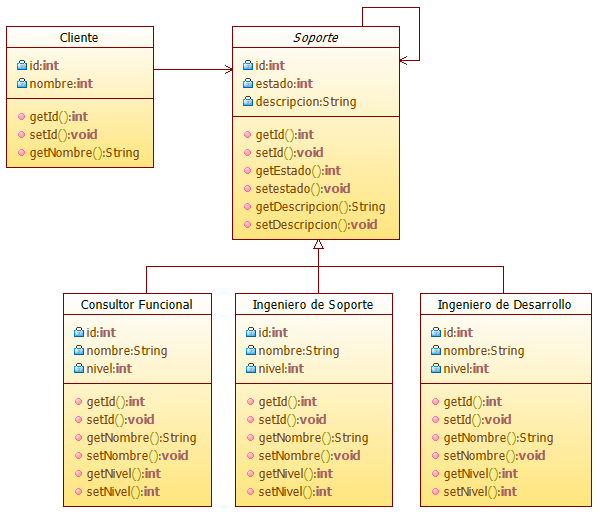
\includegraphics{figuras/1.png}
  	\captionsetup{width=.95\textwidth}
  	\caption{Organigrama Creatics}
  	\label{figura1}
  \end{figure}
  
\section{Mapa de Procesos}
  La organización con el fin de satisfacer las necesidades del cliente apoya su operación en tres procesos fundamentales: \\ \\
  \textbf{Estratégicos:} La gestión de dirección y la mejora continua dentro de su funcionamiento establecen las políticas y lineamientos que permiten llevar a cabo la misión. \\
  \textbf{Misionales:} Estos procesos llevan a cabo las operaciones orientadas a la satisfacción de las necesidades de los clientes. \\
  \textbf{Apoyo:} Son los procesos que brindan soporte a la gestión de los procesos estratégicos y misionales.

  \begin{figure}[!h]
  	\centering
  	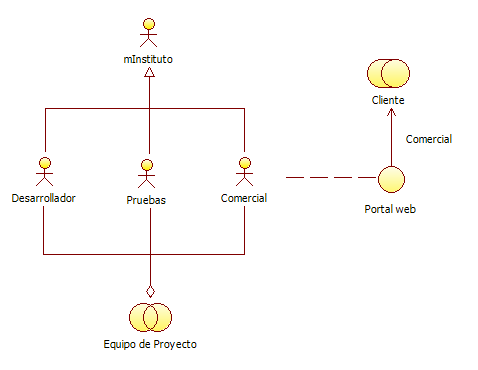
\includegraphics[scale=0.85]{figuras/2.png}
  	\captionsetup{width=.95\textwidth}
  	\caption{Mapa de Procesos}
  	\label{figura2}
  \end{figure}